\documentclass{article}\usepackage[]{graphicx}\usepackage[]{color}
% maxwidth is the original width if it is less than linewidth
% otherwise use linewidth (to make sure the graphics do not exceed the margin)
\makeatletter
\def\maxwidth{ %
  \ifdim\Gin@nat@width>\linewidth
    \linewidth
  \else
    \Gin@nat@width
  \fi
}
\makeatother

\definecolor{fgcolor}{rgb}{0.345, 0.345, 0.345}
\newcommand{\hlnum}[1]{\textcolor[rgb]{0.686,0.059,0.569}{#1}}%
\newcommand{\hlstr}[1]{\textcolor[rgb]{0.192,0.494,0.8}{#1}}%
\newcommand{\hlcom}[1]{\textcolor[rgb]{0.678,0.584,0.686}{\textit{#1}}}%
\newcommand{\hlopt}[1]{\textcolor[rgb]{0,0,0}{#1}}%
\newcommand{\hlstd}[1]{\textcolor[rgb]{0.345,0.345,0.345}{#1}}%
\newcommand{\hlkwa}[1]{\textcolor[rgb]{0.161,0.373,0.58}{\textbf{#1}}}%
\newcommand{\hlkwb}[1]{\textcolor[rgb]{0.69,0.353,0.396}{#1}}%
\newcommand{\hlkwc}[1]{\textcolor[rgb]{0.333,0.667,0.333}{#1}}%
\newcommand{\hlkwd}[1]{\textcolor[rgb]{0.737,0.353,0.396}{\textbf{#1}}}%
\let\hlipl\hlkwb

\usepackage{framed}
\makeatletter
\newenvironment{kframe}{%
 \def\at@end@of@kframe{}%
 \ifinner\ifhmode%
  \def\at@end@of@kframe{\end{minipage}}%
  \begin{minipage}{\columnwidth}%
 \fi\fi%
 \def\FrameCommand##1{\hskip\@totalleftmargin \hskip-\fboxsep
 \colorbox{shadecolor}{##1}\hskip-\fboxsep
     % There is no \\@totalrightmargin, so:
     \hskip-\linewidth \hskip-\@totalleftmargin \hskip\columnwidth}%
 \MakeFramed {\advance\hsize-\width
   \@totalleftmargin\z@ \linewidth\hsize
   \@setminipage}}%
 {\par\unskip\endMakeFramed%
 \at@end@of@kframe}
\makeatother

\definecolor{shadecolor}{rgb}{.97, .97, .97}
\definecolor{messagecolor}{rgb}{0, 0, 0}
\definecolor{warningcolor}{rgb}{1, 0, 1}
\definecolor{errorcolor}{rgb}{1, 0, 0}
\newenvironment{knitrout}{}{} % an empty environment to be redefined in TeX

\usepackage{alltt}
\PassOptionsToPackage{unicode}{hyperref}
\PassOptionsToPackage{naturalnames}{hyperref}
\usepackage{fullpage}
\usepackage[T2A]{fontenc}
\usepackage[utf8]{inputenc}
\usepackage[russian]{babel}
\usepackage{mathrsfs}
\usepackage{amsfonts}
\usepackage{amsmath }
\IfFileExists{upquote.sty}{\usepackage{upquote}}{}
\begin{document}
\title{Отчет по домашнему заданию}
\pretitle{\vspace{\droptitle}\centering\huge}
\posttitle{\par}
\author{Фахртдинов Т. А.}


\maketitle
Восьмая задача. 
Исследование зависимости между количественными признаками.

Вариант 3.
\begin{knitrout}
\definecolor{shadecolor}{rgb}{0.969, 0.969, 0.969}\color{fgcolor}\begin{kframe}
\begin{alltt}
\hlstd{h} \hlkwb{<-} \hlkwd{c}\hlstd{(}\hlnum{1.1}\hlstd{,} \hlnum{4.6}\hlstd{,} \hlnum{0.7}\hlstd{,} \hlnum{4.0}\hlstd{,} \hlnum{0.7}\hlstd{,} \hlnum{27.6}\hlstd{,} \hlnum{20.9}\hlstd{,} \hlnum{55.6}\hlstd{,} \hlnum{69.0}\hlstd{,} \hlnum{23.0}\hlstd{,} \hlnum{19.5}\hlstd{,} \hlnum{8.9}\hlstd{,} \hlnum{50.4}\hlstd{,}
       \hlnum{39.9}\hlstd{,} \hlnum{20.7}\hlstd{,} \hlnum{26.6}\hlstd{,} \hlnum{13.9}\hlstd{,} \hlnum{23.6}\hlstd{,} \hlnum{16.2}\hlstd{,} \hlnum{29.9}\hlstd{,} \hlnum{13.9}\hlstd{,} \hlnum{65.2}\hlstd{,} \hlnum{31.4}\hlstd{,} \hlnum{26.0}\hlstd{,} \hlnum{25.0}\hlstd{)}
\hlstd{t} \hlkwb{<-} \hlkwd{c}\hlstd{(}\hlnum{73.2}\hlstd{,} \hlnum{71.9}\hlstd{,} \hlnum{76.4}\hlstd{,} \hlnum{72.1}\hlstd{,} \hlnum{71.9}\hlstd{,} \hlnum{83.5}\hlstd{,} \hlnum{85.9}\hlstd{,} \hlnum{85}\hlstd{,} \hlnum{82.3}\hlstd{,} \hlnum{84.5}\hlstd{,} \hlnum{85.3}\hlstd{,} \hlnum{85.3}\hlstd{,}
       \hlnum{84.1}\hlstd{,} \hlnum{74.3}\hlstd{,} \hlnum{71}\hlstd{,} \hlnum{69.5}\hlstd{,} \hlnum{59.1}\hlstd{,} \hlnum{73.1}\hlstd{,} \hlnum{75.7}\hlstd{,} \hlnum{81.9}\hlstd{,} \hlnum{62.1}\hlstd{,} \hlnum{72.6}\hlstd{,} \hlnum{72.6}\hlstd{,} \hlnum{77.9}\hlstd{,} \hlnum{77.7}\hlstd{)}
\end{alltt}
\end{kframe}
\end{knitrout}
\textbf{Получаем оценки параметров линейной регрессии.}
\begin{knitrout}
\definecolor{shadecolor}{rgb}{0.969, 0.969, 0.969}\color{fgcolor}\begin{kframe}
\begin{alltt}
\hlstd{n} \hlkwb{<-} \hlkwd{length}\hlstd{(h)}
\hlstd{beta} \hlkwb{<-} \hlstd{(}\hlkwd{sum}\hlstd{(h} \hlopt{*} \hlstd{t)} \hlopt{-} \hlstd{n} \hlopt{*} \hlkwd{mean}\hlstd{(h)} \hlopt{*} \hlkwd{mean}\hlstd{(t))} \hlopt{/}
        \hlstd{(}\hlkwd{sum}\hlstd{(h} \hlopt{*} \hlstd{h)} \hlopt{-} \hlstd{n} \hlopt{*} \hlkwd{mean}\hlstd{(h)}\hlopt{^}\hlnum{2}\hlstd{)}
\hlstd{alpha} \hlkwb{<-} \hlkwd{mean}\hlstd{(t)} \hlopt{-} \hlstd{beta} \hlopt{*} \hlkwd{mean}\hlstd{(h)}
\end{alltt}
\end{kframe}
\end{knitrout}
Коэффициенты $\alpha$, $\beta$ соответственно равны:
\begin{knitrout}
\definecolor{shadecolor}{rgb}{0.969, 0.969, 0.969}\color{fgcolor}\begin{kframe}
\begin{verbatim}
## [1] 73.3662933  0.1208841
\end{verbatim}
\end{kframe}
\end{knitrout}
\textbf{Проверим значимость оценок:}
\begin{knitrout}
\definecolor{shadecolor}{rgb}{0.969, 0.969, 0.969}\color{fgcolor}\begin{kframe}
\begin{alltt}
\hlstd{Y} \hlkwb{<-} \hlstd{alpha} \hlopt{+} \hlstd{beta} \hlopt{*} \hlstd{h}
\hlstd{Qe} \hlkwb{<-} \hlkwd{sum}\hlstd{((t} \hlopt{-} \hlstd{Y)}\hlopt{^}\hlnum{2}\hlstd{)}
\hlstd{S2} \hlkwb{<-} \hlstd{Qe} \hlopt{/} \hlstd{(n} \hlopt{-} \hlnum{2}\hlstd{)}
\hlstd{S2.alpha} \hlkwb{<-} \hlstd{S2} \hlopt{*} \hlkwd{sum}\hlstd{(h} \hlopt{*} \hlstd{h)} \hlopt{/} \hlstd{(n} \hlopt{*} \hlkwd{sum}\hlstd{((h} \hlopt{-} \hlkwd{mean}\hlstd{(h))}\hlopt{^}\hlnum{2}\hlstd{))}
\hlstd{S2.beta} \hlkwb{<-} \hlstd{S2} \hlopt{/} \hlkwd{sum}\hlstd{((h} \hlopt{-} \hlkwd{mean}\hlstd{(h))}\hlopt{^}\hlnum{2}\hlstd{)}
\hlstd{T_a} \hlkwb{<-} \hlstd{alpha} \hlopt{/} \hlkwd{sqrt}\hlstd{(S2.alpha)}
\hlstd{T_b} \hlkwb{<-} \hlstd{beta} \hlopt{/} \hlkwd{sqrt}\hlstd{(S2.beta)}
\end{alltt}
\end{kframe}
\end{knitrout}
Значения критерия и p-value, для $\alpha$ и $\beta$ соответственно:
\begin{knitrout}
\definecolor{shadecolor}{rgb}{0.969, 0.969, 0.969}\color{fgcolor}\begin{kframe}
\begin{verbatim}
## [1] 31.44714  0.00000
## [1] 1.6049144 0.1221572
\end{verbatim}
\end{kframe}
\end{knitrout}

\newpage
Найдем значение параметров с помощью встроенной функции:
\begin{knitrout}
\definecolor{shadecolor}{rgb}{0.969, 0.969, 0.969}\color{fgcolor}\begin{kframe}
\begin{alltt}
\hlkwd{summary}\hlstd{(}\hlkwd{lm}\hlstd{(t}\hlopt{~}\hlstd{h))}
\end{alltt}
\begin{verbatim}
## 
## Call:
## lm(formula = t ~ h)
## 
## Residuals:
##      Min       1Q   Median       3Q      Max 
## -15.9466  -3.8896   0.3754   4.9125  10.8578 
## 
## Coefficients:
##             Estimate Std. Error t value Pr(>|t|)    
## (Intercept) 73.36629    2.33300  31.447   <2e-16 ***
## h            0.12088    0.07532   1.605    0.122    
## ---
## Signif. codes:  0 '***' 0.001 '**' 0.01 '*' 0.05 '.' 0.1 ' ' 1
## 
## Residual standard error: 7.023 on 23 degrees of freedom
## Multiple R-squared:  0.1007,	Adjusted R-squared:  0.06161 
## F-statistic: 2.576 on 1 and 23 DF,  p-value: 0.1222
\end{verbatim}
\end{kframe}
\end{knitrout}
Полученные значения параметров совпадают со значениями, полученными нами. Так же, полученные значения критериев и p-value совпадают с полученными нами.

\newline

$p-value_{\alpha} < 0.05$, отклоняем гипотезу о равенстве коэффициента нулю.

$p-value_{\beta} > 0.05$, нет оснований отклонить гипотезу о равенстве коэффициента нулю.

\newline

\textbf{На одном графике строим двумерную диаграмму признаков и проводим линию регрессии.}
\begin{knitrout}
\definecolor{shadecolor}{rgb}{0.969, 0.969, 0.969}\color{fgcolor}\begin{kframe}
\begin{alltt}
\hlstd{step} \hlkwb{<-} \hlkwd{seq}\hlstd{(}\hlkwd{min}\hlstd{(h),} \hlkwd{max}\hlstd{(h),} \hlkwc{by} \hlstd{=} \hlnum{0.1}\hlstd{)}
\hlstd{Y} \hlkwb{<-} \hlstd{alpha} \hlopt{+} \hlstd{beta}\hlopt{*}\hlstd{step}
\hlstd{S} \hlkwb{<-} \hlkwd{sqrt}\hlstd{(S2}\hlopt{*}\hlstd{(} \hlnum{1}\hlopt{/}\hlstd{n} \hlopt{+} \hlstd{(step} \hlopt{-} \hlkwd{mean}\hlstd{(h))}\hlopt{^}\hlnum{2}\hlopt{/}\hlkwd{sum}\hlstd{((h} \hlopt{-} \hlkwd{mean}\hlstd{(h))}\hlopt{^}\hlnum{2}\hlstd{)))}
\hlstd{confInt1} \hlkwb{<-} \hlstd{Y} \hlopt{-} \hlkwd{qt}\hlstd{(}\hlnum{1}\hlopt{-}\hlnum{0.05}\hlopt{/}\hlnum{2}\hlstd{, n} \hlopt{-} \hlnum{2}\hlstd{)} \hlopt{*} \hlstd{S}
\hlstd{confInt2} \hlkwb{<-} \hlstd{Y} \hlopt{+} \hlkwd{qt}\hlstd{(}\hlnum{1}\hlopt{-}\hlnum{0.05}\hlopt{/}\hlnum{2}\hlstd{, n} \hlopt{-} \hlnum{2}\hlstd{)} \hlopt{*} \hlstd{S}
\hlstd{confInt} \hlkwb{<-} \hlkwd{cbind}\hlstd{(confInt1, confInt2, Y)}
\hlkwd{matplot}\hlstd{(step,}
\hlstd{confInt,} \hlkwc{col}\hlstd{=}\hlkwd{c}\hlstd{(}\hlstr{"blue"}\hlstd{,}\hlstr{"blue"}\hlstd{,}\hlstr{"red"}\hlstd{),}\hlkwc{lty}\hlstd{=}\hlkwd{c}\hlstd{(}\hlnum{2}\hlstd{,}\hlnum{2}\hlstd{,}\hlnum{1}\hlstd{),}
\hlkwc{type}\hlstd{=} \hlstr{"l"}\hlstd{,} \hlkwc{ylab} \hlstd{=} \hlstr{"t"}\hlstd{,} \hlkwc{xlab} \hlstd{=} \hlstr{"h"}\hlstd{)}
\hlkwd{points}\hlstd{(h, t,} \hlkwc{pch} \hlstd{=} \hlnum{19}\hlstd{,} \hlkwc{cex} \hlstd{=} \hlnum{0.5}\hlstd{)}
\end{alltt}
\end{kframe}
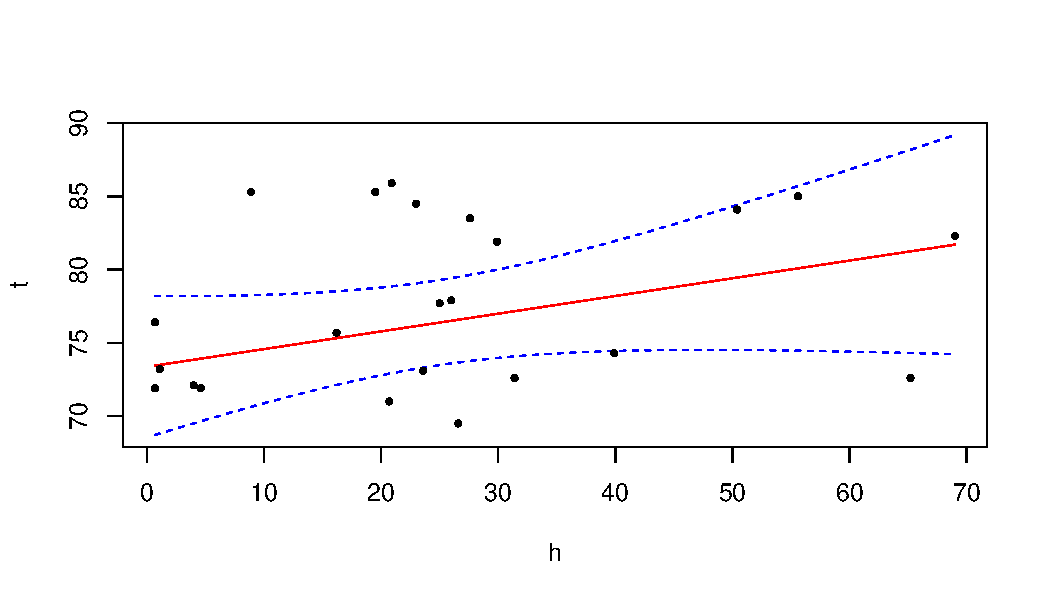
\includegraphics[width=\maxwidth]{figure/unnamed-chunk-7-1} 

\end{knitrout}

Теперь воспользуемся функцией пакета ggplot, для построения:

\begin{knitrout}
\definecolor{shadecolor}{rgb}{0.969, 0.969, 0.969}\color{fgcolor}
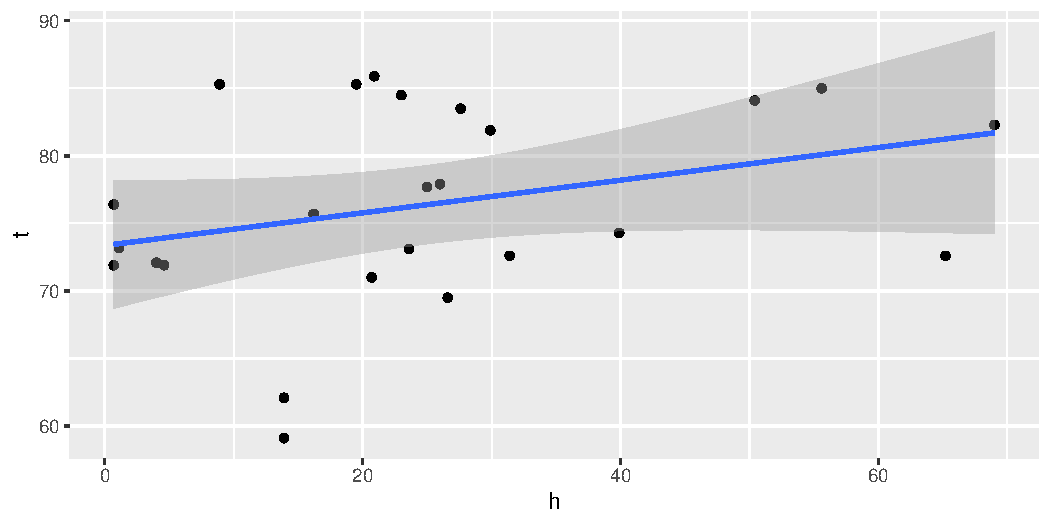
\includegraphics[width=\maxwidth]{figure/unnamed-chunk-8-1} 

\end{knitrout}

\newpage

\textbf{Вычислим коэффициенты корреляции и детерминации.}

Коэффициент детерминации:
\begin{knitrout}
\definecolor{shadecolor}{rgb}{0.969, 0.969, 0.969}\color{fgcolor}\begin{kframe}
\begin{alltt}
\hlstd{Q} \hlkwb{<-} \hlkwd{sum}\hlstd{((t} \hlopt{-} \hlkwd{mean}\hlstd{(t))}\hlopt{^}\hlnum{2}\hlstd{)}
\hlstd{R_2} \hlkwb{<-} \hlnum{1} \hlopt{-} \hlstd{Qe} \hlopt{/} \hlstd{Q}
\hlstd{R_2}
\end{alltt}
\begin{verbatim}
## [1] 0.1007106
\end{verbatim}
\end{kframe}
\end{knitrout}
Коэффициент корреляции:
\begin{knitrout}
\definecolor{shadecolor}{rgb}{0.969, 0.969, 0.969}\color{fgcolor}\begin{kframe}
\begin{alltt}
\hlstd{rho} \hlkwb{<-} \hlkwd{sum}\hlstd{((h} \hlopt{-} \hlkwd{mean}\hlstd{(h))} \hlopt{*} \hlstd{(t} \hlopt{-} \hlkwd{mean}\hlstd{(t)))}
\hlstd{rho} \hlkwb{<-} \hlstd{rho} \hlopt{/} \hlstd{(}\hlkwd{sqrt}\hlstd{(}\hlkwd{sum}\hlstd{((h} \hlopt{-} \hlkwd{mean}\hlstd{(h))}\hlopt{^}\hlnum{2}\hlstd{))} \hlopt{*} \hlkwd{sqrt}\hlstd{(}\hlkwd{sum}\hlstd{((t} \hlopt{-} \hlkwd{mean}\hlstd{(t))}\hlopt{^}\hlnum{2}\hlstd{)))}
\hlstd{rho}
\end{alltt}
\begin{verbatim}
## [1] 0.3173494
\end{verbatim}
\end{kframe}
\end{knitrout}

\textbf{Значимость коэффициента корреляции:}

Проверяется гипотеза $H_0$: $\rho = 0$
\begin{knitrout}
\definecolor{shadecolor}{rgb}{0.969, 0.969, 0.969}\color{fgcolor}\begin{kframe}
\begin{alltt}
\hlstd{T_rho}\hlkwb{<-} \hlstd{rho} \hlopt{*} \hlstd{(n} \hlopt{-} \hlnum{2}\hlstd{)} \hlopt{/} \hlkwd{sqrt}\hlstd{(}\hlnum{1} \hlopt{-} \hlstd{rho}\hlopt{^}\hlnum{2}\hlstd{)}
\hlstd{pval_rho} \hlkwb{<-} \hlnum{2} \hlopt{*} \hlkwd{min}\hlstd{(}\hlnum{1} \hlopt{-} \hlkwd{pt}\hlstd{(T_rho, n} \hlopt{-} \hlnum{2}\hlstd{),} \hlkwd{pt}\hlstd{(T_rho, n} \hlopt{-} \hlnum{2}\hlstd{))}
\end{alltt}
\end{kframe}
\end{knitrout}
Значение критерия и p-value:
\begin{knitrout}
\definecolor{shadecolor}{rgb}{0.969, 0.969, 0.969}\color{fgcolor}\begin{kframe}
\begin{verbatim}
## [1] 7.696899e+00 8.266966e-08
\end{verbatim}
\end{kframe}
\end{knitrout}
8.266966e-08 < 0.05, отклоняем гипотезу о равенстве коэффициента корреляции нулю.

\textbf{Значимость коэффициента детерминации:}

Проверяется гипотеза $H_0$: $R^2 = 0$
\begin{knitrout}
\definecolor{shadecolor}{rgb}{0.969, 0.969, 0.969}\color{fgcolor}\begin{kframe}
\begin{alltt}
\hlstd{T_r2}\hlkwb{<-} \hlkwd{sqrt}\hlstd{(R_2)} \hlopt{*} \hlstd{(n} \hlopt{-} \hlnum{2}\hlstd{)} \hlopt{/} \hlkwd{sqrt}\hlstd{(}\hlnum{1} \hlopt{-} \hlstd{R_2)}
\hlstd{pval_r2} \hlkwb{<-} \hlnum{2} \hlopt{*} \hlkwd{min}\hlstd{(}\hlnum{1} \hlopt{-} \hlkwd{pt}\hlstd{(T_r2, n} \hlopt{-} \hlnum{2}\hlstd{),} \hlkwd{pt}\hlstd{(T_r2, n} \hlopt{-} \hlnum{2}\hlstd{))}
\end{alltt}
\end{kframe}
\end{knitrout}
Значение критерия и p-value:
\begin{knitrout}
\definecolor{shadecolor}{rgb}{0.969, 0.969, 0.969}\color{fgcolor}\begin{kframe}
\begin{verbatim}
## [1] 7.696899e+00 8.266966e-08
\end{verbatim}
\end{kframe}
\end{knitrout}
8.266966e-08 < 0.05, отклоняем гипотезу о равенстве коэффициента детерминации нулю. Что ожидаемо, так как проверка гипотезы о равенстве коэффициента детерминации нулю эквивалентна проверке гипотезы о равенстве нулю коэффициента корреляции.

\end{document}
